\documentclass[11pt]{article}%

\usepackage[top=1in, bottom=1in, right=1in, left=1in]{geometry}
\usepackage{listings}
\usepackage{xcolor}
\usepackage{titlesec}
\definecolor{lgray}{HTML}{FCFCFC}
\usepackage{graphicx}
\usepackage{rotating}
\usepackage{float}
\usepackage{grffile}

\usepackage[utf8]{inputenc}

\titleformat*{\section}{\Huge\centering\bf}
\titleformat*{\subsection}{\Large\bfseries}

\usepackage{underscore}

\usepackage{pgffor}%
\newcommand*{\ListHpp}{%
code/ui.hpp
}%
\newcommand*{\ListCpp}{%
code/interact.cpp,
code/uibase.cpp,
code/frame.cpp,
code/box.cpp,
code/validation.cpp,
code/llayout.cpp,
code/button.cpp,
code/textbox.cpp,
code/infotbox.cpp
}%
\newcommand*{\ListOthers}{%

}%
%

\begin{document}%

\lstset{ 
    language=C++, % choose the language of the code
    basicstyle=\fontfamily{pcr}\selectfont\footnotesize,
    numbers=left, % where to put the line-numbers
    numberstyle=\tiny, % the size of the fonts that are used for the line-numbers     
    backgroundcolor=\color{lgray},
    showspaces=false, % show spaces adding particular underscores
    showstringspaces=false, % underline spaces within strings
    showtabs=false, % show tabs within strings adding particular underscores
    frame=none, % adds a frame around the code
    tabsize=4, % sets default tabsize to 2 spaces
    rulesepcolor=\color{gray},
    breaklines=true, % sets automatic line breaking
    breakatwhitespace=false, 
}

\begin{titlepage}
    \begin{center}
        \vspace*{3cm}
        
        \Huge
        \textbf{LHospital}
        
        \vspace{0.5cm}
        \LARGE
        A \textit{Turbo} C++ project \\
        A basic management system for a general hospital
        \vfill
        
        \textbf
     	{
        \begin{tabular}{ r c }
        	Arpit Saxena & 9151996\\
        	Anirudh Panigrahi & 9151993\\
        	Sankalp Gambhir & 9152014
        \end{tabular}
        }
        
        \vfill
        
        
    \end{center}
\end{titlepage}

\newpage

\topskip0pt
\vspace*{\fill}
\centering\Large\textit{This page has been intentionally left blank.}
\vspace*{\fill}
%

\newpage

\tableofcontents

\newpage

\section{Diagrams}

\subsection{ER diagrams}

\begin{enumerate}

\item{\large{ Hospital }}
\\
\begin{figure}[H]

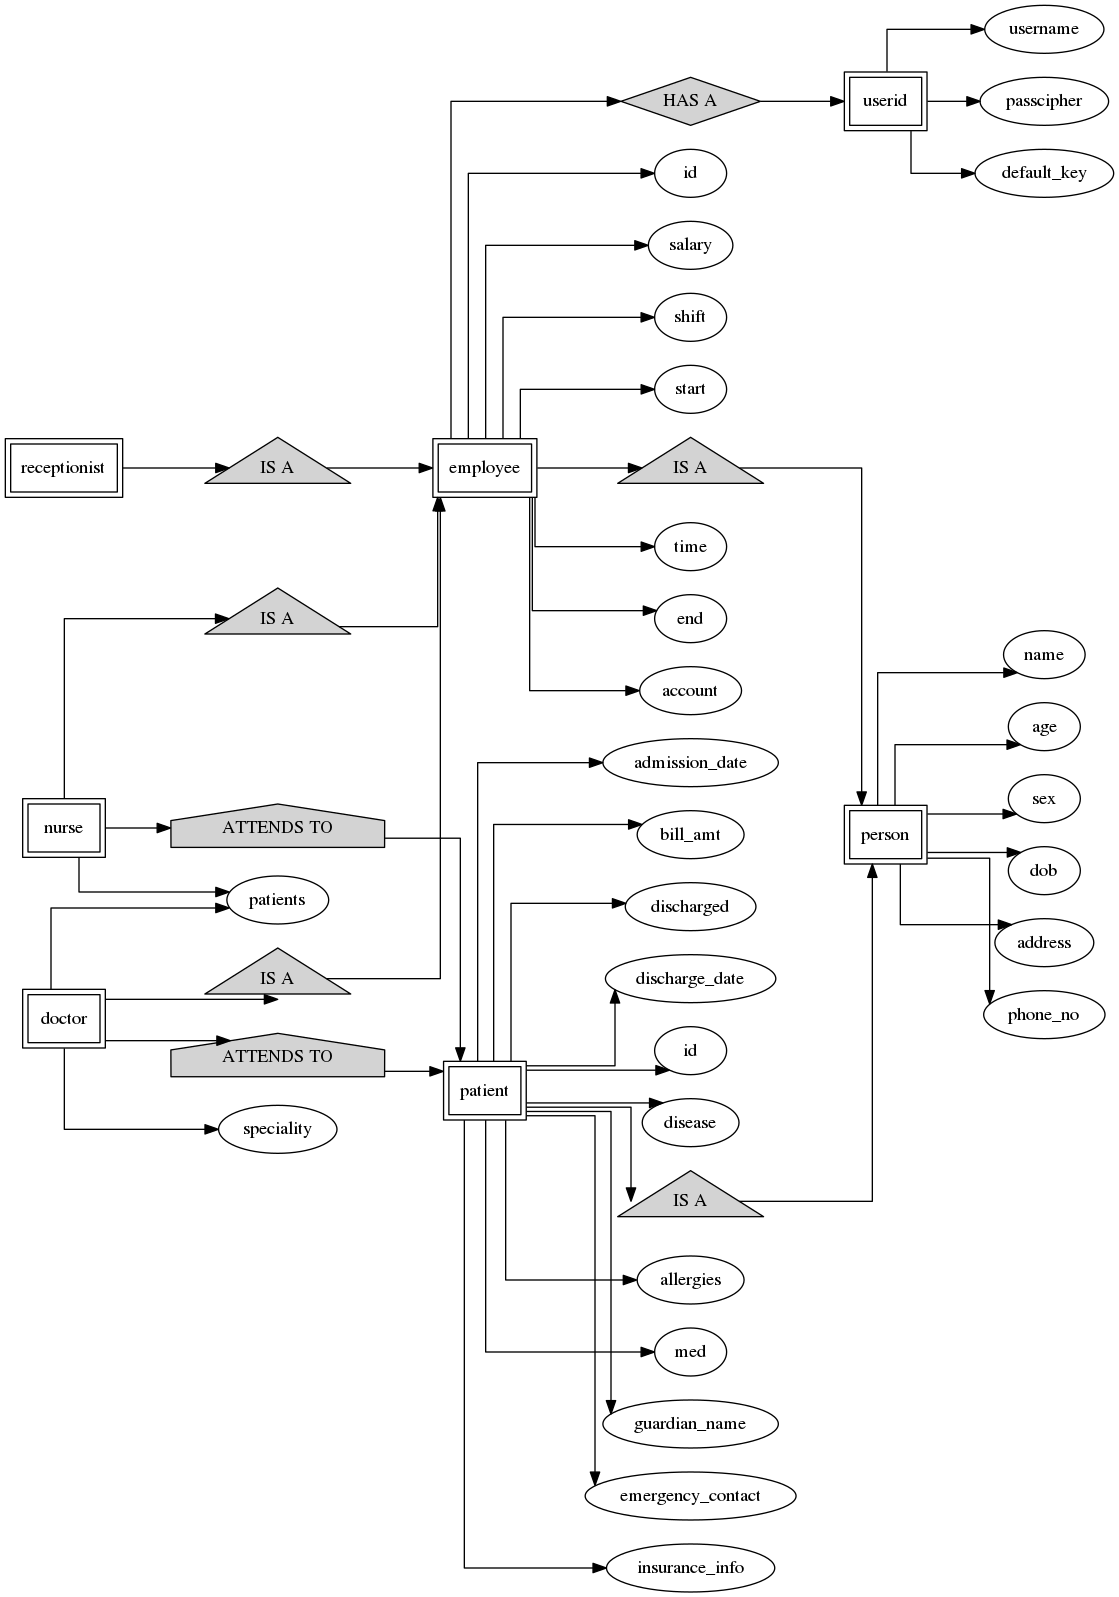
\includegraphics[width = 0.81\textwidth]{fig/hosp.png}

\end{figure}

\item{\large{ User interface }}
\\
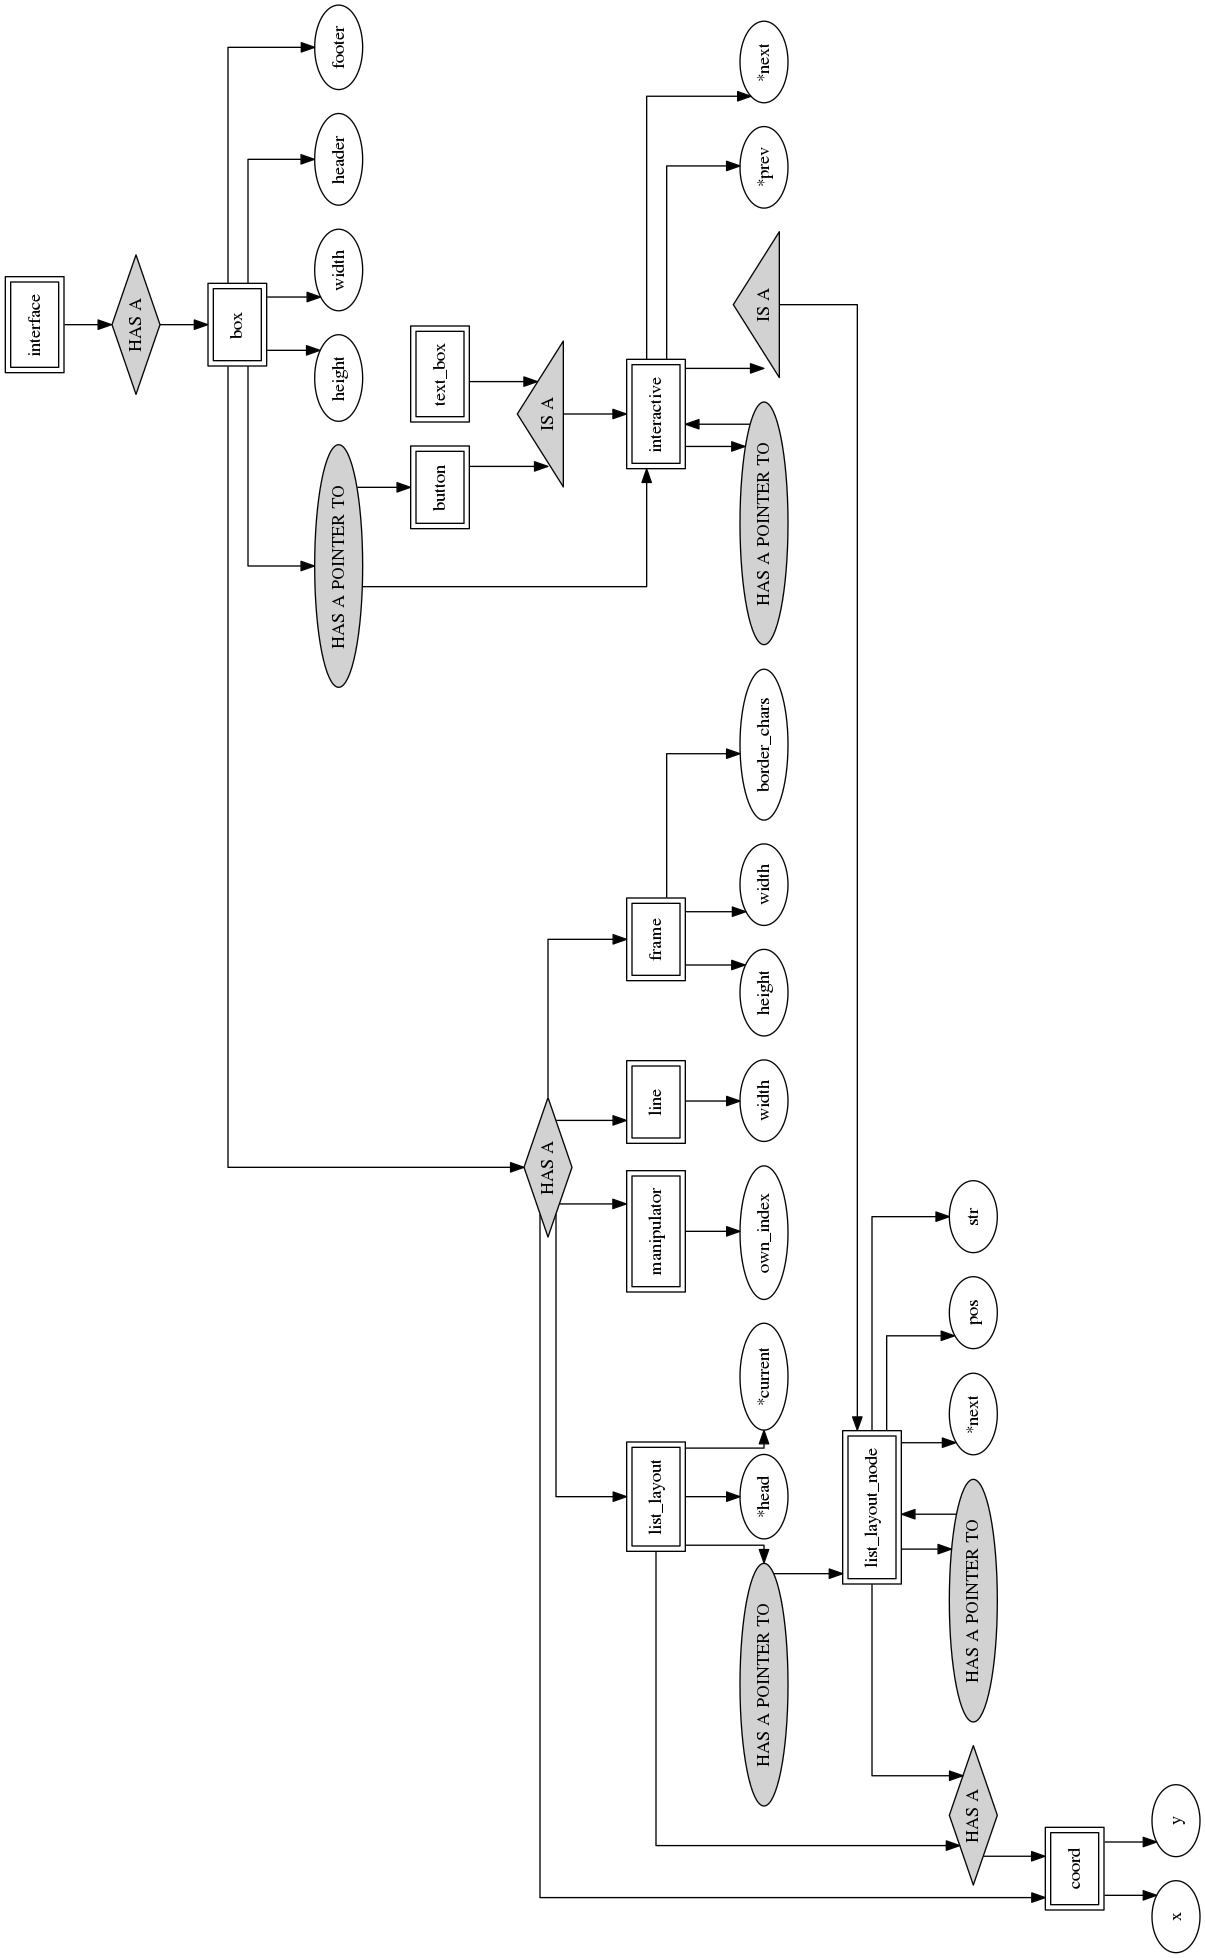
\includegraphics[width = 0.8\textwidth]{fig/uir.png}
\\
\small\textbf{Note: The figure included has been rotated}


\end{enumerate}

\newpage

\begin{figure}[H]

\subsection{Flowchart of main()}

\begin{center}

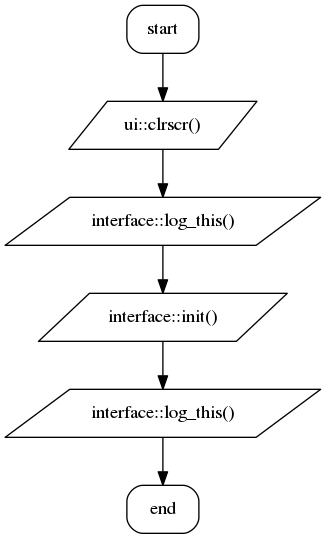
\includegraphics[width = 8.5cm]{fig/main.png}

\end{center}

\end{figure}

\newpage

\section{Source Code}

\subsection{Header files}

\begin{enumerate}

\foreach \c in \ListHpp {%
    \item{\large\c}%
    \lstinputlisting{\c}
}%

\end{enumerate}
\newpage
\subsection{C++ files (.cpp)}

\begin{enumerate}

\foreach \c in \ListCpp {%
    \item{\large\c}%
    \lstinputlisting{\c}
    \vspace{0.3cm}
}%

\end{enumerate}

\newpage
\subsection{Data files}

\begin{enumerate}

\foreach \c in \ListOthers {%
    \item{\large\c}%
}%

\end{enumerate}

\newpage
\section{Output}


\foreach \c in \ListOutput {%
    \includegraphics[width = \textwidth]{\c}
    \vspace{0.3cm}
}

\end{document}
